\documentclass[a4paper,12pt]{article}% article ,book, report, standalone
%%preamble
\usepackage{blindtext}
\usepackage{fullpage}
\usepackage{amsmath}%for align nonumber
\usepackage{xcolor}
\usepackage{soul}
\usepackage{graphicx}




\begin{document}
%main matter
\section{Intro to math}

\subsection{Equations}
\begin{figure}

\includegraphics{./01.png}
\caption{demo caption of figure}
\end{figure}


\begin{figure}

\includegraphics{./img/01.png}
\caption{demo caption of figure}
\end{figure}

\begin{figure}
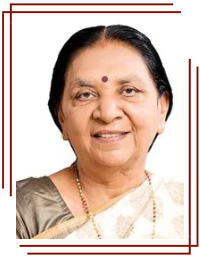
\includegraphics{./img/02.jpg}
\caption{demo caption of figure}
\end{figure}


\hl{text should be highlighted}
\so{text should be highlighted}
\ul{text should be highlighted}
\hl{text should be highlighted}
\begin{equation}
a=b
\end{equation}



\begin{equation}
a=\int x dx\\ abc
\end{equation}

\blindtext
\begin{align}
a=&\int_0^{10} x dx+\lim_{x=0} x+ \sin x+\frac{d x}{d y}\nonumber\\=&cb\\
=&y\nonumber\\
=&b\label{eqn:demo1}
\end{align}

{\color{red}

\blindtext as $e=mc^2$ in \eqref{eqn:demo1}
}

\textcolor{blue}{
\blindtext as $e=mc^2$ in \eqref{eqn:demo1}
}





\begin{align}
a=\int_)^\infty x \partial x + e^2+\delta\Delta\omega\Omega\alpha
\end{align}







\begin{equation}
a=\left[x\times\left(a\left\{\frac{a}{b}\right\}\right)\right]
\end{equation}



\begin{equation}
a=\left\{\frac{a}{b}\right\}
\end{equation}



\begin{equation}
a=b
\end{equation}





\end{document}


% \ref \label